\documentclass{beamer}
\usepackage[utf8]{inputenc}

\usetheme{Madrid}
\usecolortheme{default}
\usepackage{amsmath,amssymb,amsfonts,amsthm}
\usepackage{mathtools}
\usepackage{txfonts}
\usepackage{tkz-euclide}
\usepackage{listings}
\usepackage{adjustbox}
\usepackage{array}
\usepackage{gensymb}
\usepackage{tabularx}
\usepackage{gvv}
\usepackage{lmodern}
\usepackage{circuitikz}
\usepackage{tikz}
\lstset{literate={·}{{$\cdot$}}1 {λ}{{$\lambda$}}1 {→}{{$\to$}}1}
\usepackage{graphicx}

\setbeamertemplate{page number in head/foot}[totalframenumber]

\usepackage{tcolorbox}
\tcbuselibrary{minted,breakable,xparse,skins}



\definecolor{bg}{gray}{0.95}
\DeclareTCBListing{mintedbox}{O{}m!O{}}{%
  breakable=true,
  listing engine=minted,
  listing only,
  minted language=#2,
  minted style=default,
  minted options={%
    linenos,
    gobble=0,
    breaklines=true,
    breakafter=,,
    fontsize=\small,
    numbersep=8pt,
    #1},
  boxsep=0pt,
  left skip=0pt,
  right skip=0pt,
  left=25pt,
  right=0pt,
  top=3pt,
  bottom=3pt,
  arc=5pt,
  leftrule=0pt,
  rightrule=0pt,
  bottomrule=2pt,
  toprule=2pt,
  colback=bg,
  colframe=orange!70,
  enhanced,
  overlay={%
    \begin{tcbclipinterior}
    \fill[orange!20!white] (frame.south west) rectangle ([xshift=20pt]frame.north west);
    \end{tcbclipinterior}},
  #3,
}
\lstset{
    language=C,
    basicstyle=\ttfamily\small,
    keywordstyle=\color{blue},
    stringstyle=\color{orange},
    commentstyle=\color{green!60!black},
    numbers=left,
    numberstyle=\tiny\color{gray},
    breaklines=true,
    showstringspaces=false,
}
%------------------------------------------------------------
%This block of code defines the information to appear in the
%Title page
\title %optional
{5.13.104}
\date{September 5,2025}
%\subtitle{A short story}

\author % (optional)
{AI25BTECH11035-SUJAL RAJANI}
\begin{document}
\frame{\titlepage}
\begin{frame}{Question}
\textbf{QUESTION}
\\
Let $\vec{R}^2$ denote the Euclidean space . Let S={($a,b,c$):$a,b,c$$\epsilon$$\vec{R}$,$ax^2+2bxy+cy^2>0$$\forall(x,y)\epsilon\vec{R}^2-{(0,0)}$}.Then which of the following statement is (are) TRUE ?
\\
  (a) (2,$\frac{7}{2}$,6)$\epsilon$S
  \\
  (b) IF (3,b,$\frac{1}{12}$)$\epsilon$S,then $|2b|<1 $.
  \\
  (c)For any given ($a,b,c$)$\epsilon$S,the system of linear equations 
  \begin{align*}
      ax+by=1
      \\
      bx+cy=-1
  \end{align*}
  has a unique solution .
  \\
  (d) For any given ($a,b,c$)$\epsilon$S, the system of linear equations 
  \begin{align*}
      (a+1)x+by=0
      \\
      bx+(c+1)y=0
  \end{align*}
  has a unique solution .
\end{frame}

\begin{frame}{Theoretical Solution}
\textbf{solution}
\\
as mentioned in the question :
\\
\begin{align*}
    ax^2+2bxy+cy^2>0\forall(x,y)\epsilon\vec{R}^2-{(0,0)}
\end{align*}
let Q be a matric :
\begin{align*}
    \vec{Q}=\myvec{a&b\\b&c}
\end{align*}
then:
\begin{align*}
    ax^2+2bxy+cy^2=\myvec{x&y}\myvec{a&b\\b&c}\myvec{x\\y}
\end{align*}
for this to happen :
\\
\begin{align*}
    a>0,c>0,||\vec{Q}||=ac-b^2>0 
\end{align*}
So,S:({(a,b,c):$a>0,c>0$,$ac-b^2>0$})
\end{frame}
\begin{frame}{Theoretical solution}
option (a):
\\
$a=2>0$,c=6,b=$\dfrac{7}{2}$
\\
\begin{align*}
    ac-b^2=12-(\dfrac{7}{2})^2=-\dfrac{1}{4}<0
\end{align*}
option a is not correct .
\end{frame}

\begin{frame}{Theoretical Solution}
option b is correct :
\\
\begin{align*}
    a=3>0,ac-b^2=\dfrac{1}{4}-b^2>0,|2b|<1
\end{align*}
option b  is correct .
\end{frame}
\begin{frame}{SOLUTION}
 option c :
\\
\begin{align*}
    ax+by=1,bx+cy=-1.
    \\
    \myvec{a&b\\b&c}\vec{x}=\myvec{1\\-1}
\end{align*}
for the solution to be unique:
\\
\begin{align*}
    ||\vec{Q}||=ac-b^2\neq0.
\end{align*}
from the definition of S,$ac-b^2>0$.
\\
option c is correct .
\end{frame}
\begin{frame}{Theoretical Solution}
 option d is not correct 
\\
\begin{align*}
    (a+1)x+by=0,bx+(c+1)y=0.
\end{align*}
this type of homogeneous equation either have one solution or infinite solution .
\\
in case of one solution the solution is (0,0) which we do not get for any $$(a,b,c)\epsilon S$$.
\end{frame}

\begin{frame}{Plot}
    \begin{figure}[H]
    \centering
    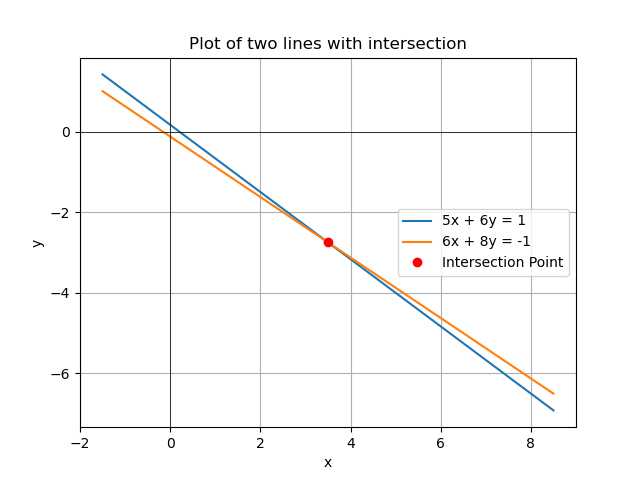
\includegraphics[width=0.6\columnwidth]{../figs1/img.png}
    \label{fig:1}
\end{figure}
\end{frame}
\begin{frame}{Plot}
    \begin{figure}[H]
    \centering
    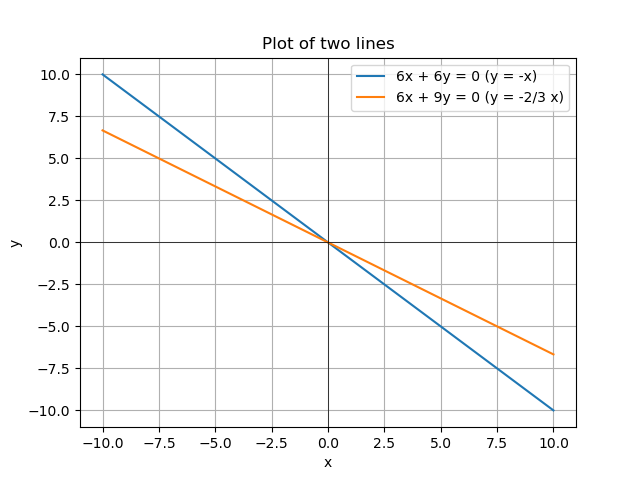
\includegraphics[width=0.6\columnwidth]{../figs2/img.png}
    \label{fig:1}
\end{figure}
\end{frame}
\end{document}